\section{Sample Control} \label{sec:Sample Control}
The sample control module is responsible for controlling the DAC and the two ADC's in the analog front end. The module will also take the samples from the ADC and store them in sample memory so the microprocessor module can retrieve them later. The module can be seen on figure \refq{fig_6_3_SampleControl}.

\begin{figure}[H]
    \centering
    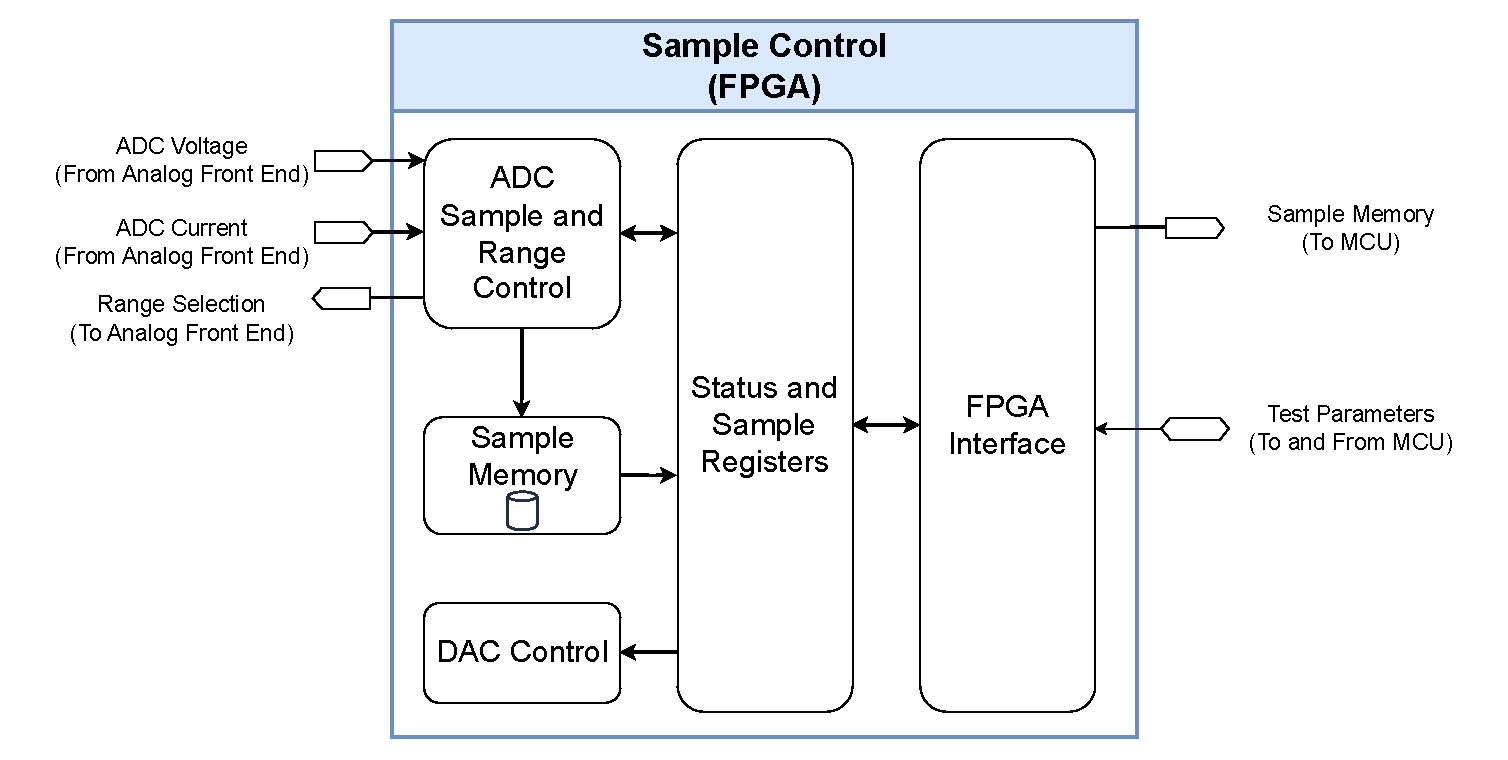
\includegraphics[clip, trim=18 0 18 0,width=0.70\textwidth]{Sections/6_SystemArchitecture/Figures/FPGA.pdf}
    \caption{The sample control module is an FPGA with external sample memory. It will control the ADC's and DAC in the analog front end. The sample control module will take samples from the ADC's and store them in memory.}
    \label{fig_6_3_SampleControl}
\end{figure}

The timing for the two sampling ADC's is critical and any mistiming will result in phase errors in the measured voltage and current waveforms. The DAC will require a significant amount of data inputs in order to produce an output in the high end of the desired frequency range of \SIQ{1}{\mega\hertz} for these reasons the \textit{sample control} module is an FPGA. The considerations for this choice can be seen in appendix \refq{App:MicrocontrollerConsiderations}. 

The sample control module is responsible for selecting the range resistors in the analog front end and adjusting the ADC amplifiers so that the ADC always sees the highest possible input signals. This will improve the ADC's SNR. The module will, before an actual test, take some test samples from the DUT in order to determine the correct range resistor. If a change of range resistor is not enough then the FPGA may adjust the gain of the ADC amplifiers. Adjusting the range resistors is preferred as the amplifiers will introduce noise into the system that will then be amplified, so, adjusting the range resistors is preferred.

The sample control module will also interface with the microprocessor module through a parallel bus. The parallel bus is the \textit{sample memory} and \textit{test parameter} signals shown on figure \refq{fig_6_3_SampleControl}. The width and details of this bus will be shown in the module interface. 